\section{Group Theory Prerequisites}
Here we list some group theory definitions and theorems used in the text.

\subsection{Basic Definitions}
\begin{definition}
	A \textit{group} $G$ is a non-empty set with a binary operation $*$, such that
	\begin{itemize}
		\item For any $g, h \in G$, we have $g * h \in G$;
		\item For any $g, h, k  \in G$, we have $(g * h) * k = g * (h * k)$;
		\item There exists an identity element $e \in G$ such that for all $g \in G$, we have $e * g = g * e = g$;
		\item For each $g \in G$, there exists an inverse element $g^{-1} \in G$ such that $g * g^{-1} = g^{-1} * g = e$. 
	\end{itemize}
\end{definition}

\begin{definition}
	A group $G$ is called \textit{abelian} if for any $g, h \in G$, we have that $g * h = h * g$. 
\end{definition}

\begin{definition}
	A \textit{subgroup} $H$ of a group $G$ is a subset of $G$ which is a group itself, denoted as $H \le G$. 
\end{definition}

\begin{definition}
	A \textit{normal subgroup} $N$ of a group $G$ is a subgroup of $G$ such that $gNg^{-1} = N$ for all $g \in G$. We denote $N \trianglelefteq G$. 
\end{definition}

\begin{definition}
	Given groups $N \trianglelefteq G$, $G / N = \{g N : g \in G\}$ is called the \textit{quotient group} of $N$, where the multiplication is defined by $g_1N g_2N = g_1g_2N$. 
\end{definition}

\begin{definition}
	Given groups $G$ and $H$, a group homomorphism $\phi: G \to H$ is a function such that $\phi(xy) = \phi(x) \phi(y)$ for any $x, y \in G$. It can be shown that $\phi(e) = e$ and $\phi(x^{-1}) = \phi(x) ^ {-1}$. The \textit{image} of $\phi$ is $\Img(\phi) = \{\phi(x) : x\in G\}$ and the \textit{kernel} of $\phi$ is $\Ker(\phi) = \{x \in G : \phi(x) = e\}$. It can be shown that $\Img(\phi) \le H$ and $\Ker(\phi) \trianglelefteq G$.  
\end{definition}

\subsection{Symmetric Groups}
\begin{definition}  \label{def:permutation}
	Given a set $X$, a \textit{permutation} of $X$ is a bijection from $X$ to $X$. All the permutations of $X$ form a group under composition, which is the \textit{permutation group} of $X$, denoted by $S_X$. In particular, when $X = \{1, \dots, n\}$, we denote $S_X$ as $S_n$ and call it a \textit{symmetric group}. $S_n$ has order $n!$. 
\end{definition}

\begin{definition}
	A permutation that is a product of an even number of transpositions is called an \textit{even permutation}. The normal subgroup of $S_n$ consisting of all even permutations is the \textit{alternating group}, denoted as $A_n$. 
\end{definition}

We look at how symmetric groups can be generated by its elements. 

\begin{theorem} \label{thm:symmetric-12-12n}
	The transposition $(12)$ and $n$-cycle $(12 \dots n)$ together generate $S_n$. 
\end{theorem}
\begin{proof}
	Consider the cyclic decomposition of each element in $S_n$, where each cyclic permutation can be written as 
	$
	(a_1a_2\dots a_k) = (a_1 a_k) \dots (a_1 a_3) (a_1 a_2). 
	$
	Note that $(ab) = (1a)(1b)(1a)$, therefore $(12), (13), \ldots (1n)$ together generate $S_n$. Also note that  
	$$(1k)=((k-1)k)\dots(34)(23)(12)(23)(34)\dots((k-1)k),$$
	therefore $(12), (23), \dots, ((n-1)n)$ together generate $S_n$. Finally note that 
	$$
	(k(k+1)) = (12\dots n)^{k-1} (12) (12\dots n)
	$$
	for $k = 2, 3, \dots n - 1$. Therefore $(12)$ and $(12 \dots n)$ together generate $S_n$. 
\end{proof}

\begin{theorem} \label{thm:symmetric-ab-12n}
	For $1 \le a < b \le n$ such that $(b - a, n) = 1$, the transposition $(ab)$ and $n$-cycle $(12 \dots n)$ together generate $S_n$.
\end{theorem}
\begin{proof}
	Let $\sigma=(12 \ldots n)$, so $\sigma^i(a) \equiv a+i \bmod n$. Therefore $\sigma^{b-a}(a) \equiv b \bmod n$, and since $1 \le b \le n$, we have $\sigma^{b-a}(a)=b$. Since $(b-a, n)=1,\langle\sigma\rangle=\left\langle\sigma^{b-a}\right\rangle$ and $\sigma^{b-a}$ is an $n$-cycle sending $a$ to $b$, so $\sigma^{b-a}$ is of the form $(a b \ldots)$. Then
	$
	\langle(a b), \sigma\rangle=\left\langle(a b), \sigma^{b-a}\right\rangle=\langle(a b),(a b \ldots)\rangle .
	$
	Relabel the numbers $1,2 \ldots, n$ so that $(a b)$ turns into $(12)$ and $(a b \ldots)$ into $(12 \ldots n)$. Therefore $\langle(a b), \sigma\rangle=S_n$ by Theorem \ref{thm:symmetric-12-12n}.
\end{proof}

\begin{theorem} \label{thm:symmetric-prime}
	For a prime number $p$, any transposition and $p$-cycle together generate $S_p$.
\end{theorem}
\begin{proof}
	Relabel the numbers so that the $p$-cycle turns into $(12 \dots p)$. Suppose the transposition turns into $(ab)$, where $1 \le a < b \le n$. Since $p$ is prime and $1 \le b - a < p$, we have $(b - a, p) = 1$. The result thus follows from Theorem \ref{thm:symmetric-ab-12n}.
\end{proof}

\subsection{Isomorphism Theorems}

\begin{theorem}[First Isomorphism Theorem] \label{thm:first-iso}
	Suppose $\phi: G \to H$ is a group homomorphism. Then its kernel $\operatorname{Ker}(\phi)$ is a normal subgroup in $G$, its image $\operatorname{Im}(\phi)$ is a subgroup in $H$, and 
	$$
	G / \operatorname{Ker}(\phi) \cong \operatorname{Im}(\phi).
	$$
\end{theorem}

\begin{theorem}[Second Isomorphism Theorem] \label{thm:second-iso}
	Suppose $H \le G$ and $J \trianglelefteq G$. Then $HJ \le G$, $H \cap J \triangleleft H$ and $$
	(HJ) / J \cong H / (H \cap J). 
	$$
\end{theorem}
\begin{theorem}[Third Isomorphism Theorem] \label{thm:third-iso}
	Suppose $H, J \trianglelefteq G$ and $H \le J$. Then $J/H \trianglelefteq G/H$ and $$
	(G/H)/(J/H) \cong G / J.    $$
\end{theorem}



\subsection{Group Actions}



\begin{definition} \label{def:action}
	Given a group $G$ and a set $X$, if there is a homomorphism
	$$
	T: G \rightarrow S_X, \quad g \mapsto T_g,
	$$
	where $T_g(x) \in X$, then the group \textit{acts} on $X$ and $X$ is a $G$-set. 
\end{definition}

\begin{definition}
	For any $x \in X$, the $G$-orbit of $x$ in $X$ is
	$$\operatorname{Orb}_G(x) = \{ y = T_g(x) : g \in G \} \subseteq X.$$

	
%	\paragraph{Stabiliser} For any $x \in X$, the stabiliser of $x$ in $G$ is 
%	$$\Stab_G(x) = \{ g \in G : T_g(x) = x \} \le G. $$
%	It is a subgroup of $G$.
\end{definition}

\begin{definition} \label{def:transitive-action}
	Given a group $G$ acting on a set $X$, $G$ acts \textit{transitively} on $X$ if for any $x \in X$, $\Orb_G(x) = X$. Equivalently, for any $x, y\in X$, there exists $g \in G$, such that $T_g(x) = y$. 
\end{definition}

\begin{theorem}[Cauchy's Theorem] \label{thm:cauchy}
	Let $p$ be a prime number. Let $G$ be a finite group such that $p$ divides the order of $G$. Then $G$ contains an element of order $p$. 
\end{theorem}

\subsection{Soluble Groups}
This is a restatement and proof of Theorem \ref{thm:soluble-main}.

\begin{theorem} \label{thm:soluble-main-appendix}
	Let $G$ be a group, $H \le G$ and $N \trianglelefteq G$. Then 
	\begin{enumerate}
		\item If $G$ is soluble, then $H$ is soluble;
		\item If $G$ is soluble, then $G / N$ is soluble; 
		\item If $N$ and $G / N$ are soluble, then $G$ is soluble. 
	\end{enumerate}
\end{theorem}
\begin{proof}
	\begin{enumerate}
		\item If $G$ is soluble, then there exists a finite series of subgroups $G_i$ of $G$ for $i = 0, 1, \dots, n$ satisfying Definition \ref{def:soluble}. Let $H_i = G_i \cap H$. Then $H$ has a series of subgroups $H_i$ such that $\{ e \} = H_0 \triangleleft H_1 \triangleleft \dots \triangleleft H_n = H.$
		For each $i = 0, 1, \dots, n - 1$, 
		$$
		\frac{H_{i+1}}{H_i} 
		= \frac{G_{i+1} \cap H}{G_i \cap (G_{i+1} \cap H)}
		\cong \frac{G_i(G_{i+1} \cap H)} {G_i}
		$$
		by Theorem \ref{thm:second-iso}, and ${G_i(G_{i+1} \cap H)}/{G_i}$ is a subgroup of the abelian group $G_{i+1} / G_{i}$. Hence $H_{i+1} / H_{i}$ is abelian and $H$ is soluble.
		\item Take $G_i$ as before. Then $G / N$ has a series
		$N/N = G_0 N / N \triangleleft G_1 N / N \triangleleft \dots \triangleleft G_n N / N  =  G / N. $
		For each $i = 0, 1, \dots, n - 1$, 
		$(G_{i+1} N / N) / (G_{i} N / N) \cong (G_{i+1} N) / (G_i N)$
		by Theorem \ref{thm:third-iso}. Then 
		$$
		\frac{G_{i+1} N}{G_i N} =\frac{G_{i+1}\left(G_i N\right)}{G_i N} \cong \frac{G_{i+1}}{G_{i+1} \cap\left(G_i N\right)} \cong \frac{G_{i+1} / G_i}{\left(G_{i+1} \cap\left(G_i N\right)\right) / G_i},
		$$
		which is a quotient of the abelian group $G_{i+1} / G_i$, so is abelian. Hence $G / N$ is soluble.
		\item There exist two series
		$$
		\begin{aligned}
			\{ e \} & =N_0 \triangleleft N_1 \triangleleft \ldots \triangleleft N_r=N, \\
			N / N & =G_0 / N \triangleleft G_1 / N \triangleleft \ldots \triangleleft G_s / N=G / N
		\end{aligned}
		$$
		with $N_{i+1} / N_{i}$ abelian for each $i = 0, 1, \dots, r-1$ and $(G_{i+1} / N)  / (G_{i} / N) \cong G_{i+1} / G_i $ abelian for each $i = 0,1, \dots, s-1$. Combining them gives the series of subgroups of $G$:
		$$
		\{ e \}=N_0 \triangleleft N_1 \triangleleft \ldots \triangleleft N_r=N=G_0 \triangleleft G_1 \triangleleft \ldots \triangleleft G_s=G .
		$$
		The quotients are either $N_{i+1} / N_i$  or $G_{i+1} / G_i$ and are all abelian. Therefore $G$ is soluble.
	\end{enumerate}
\end{proof}


\begin{definition}
	A group $G$ is \textit{simple} if it is nontrivial and its only normal subgroups are $\{ e \}$ and $G$. 
\end{definition}

\begin{theorem} \label{thm:soluble-and-simple}
	A soluble group is simple if and only if it is a cyclic group of prime order.
\end{theorem}

\begin{proof}
	Let $G$ be a soluble group and suppose $G$ is simple. Consider the series of subgroups of $G$
	$$
	\{ e \}=G_0 \triangleleft G_1 \triangleleft \ldots \triangleleft G_n=G,
	$$
	with abelian quotients, and without loss of generality we assume $G_{i+1} \neq G_i$. Since $G$ is simple, $G_{n-1}$, which is a proper normal subgroup of $G_n = G$, must be $\{ e \}$. Solubility of $G$ gives that $G_n / G_{n -1 }$ is abelian, but $G_n / G_{n - 1} = G$, and thus $G$ is abelian. Thus for any element $g \in G$, the cyclic group $\langle g\rangle$ is a normal subgroup in $G$. Hence  $G = \langle g\rangle$ for any $g \neq e$. Hence $G$ is cyclic of prime order.
	
	The converse is trivial.
\end{proof}


\begin{theorem} \label{thm:simple-alternating}
	The alternating group $A_n$ is simple when $n \ge 5$. 
\end{theorem}

\begin{proof}
    Due to the length and technical nature of the complete proof, only a concise summary is presented here. 
	Suppose that $\{ e \} \neq N \triangleleft A_n$. We can prove that $N$ must contain a $3$-cycle using case-by-case analysis. Next, we can show that if $N$ contains a $3$-cycle, then it contains all $3$-cycles. Since $A_n$ is generated by the $3$-cycles when $n \ge 3$, this means $N = A_n$.
\end{proof}

This is a restatement and proof of Theorem \ref{thm:symmetric-not-soluble}. 

\begin{theorem} \label{thm:symmetric-not-soluble-appendix}
	The symmetric group $S_n$ is not soluble when $n \ge 5$. 
\end{theorem}

\begin{proof}
	Suppose $S_n$ is soluble for $n \ge 5$. Then since $A_n \trianglelefteq S_n$, by Theorem \ref{thm:soluble-main}, $A_n$ is soluble. By Theorem \ref{thm:simple-alternating}, $A_n$ is also simple, so $A_n$ is cyclic of prime order by Theorem \ref{thm:soluble-and-simple}. But $|A_n| = n! / 2$ which obviously is not prime. Contradiction.
\end{proof}

\section{Constructions}

\FloatBarrier
\begin{figure}[!hbt]
\centering
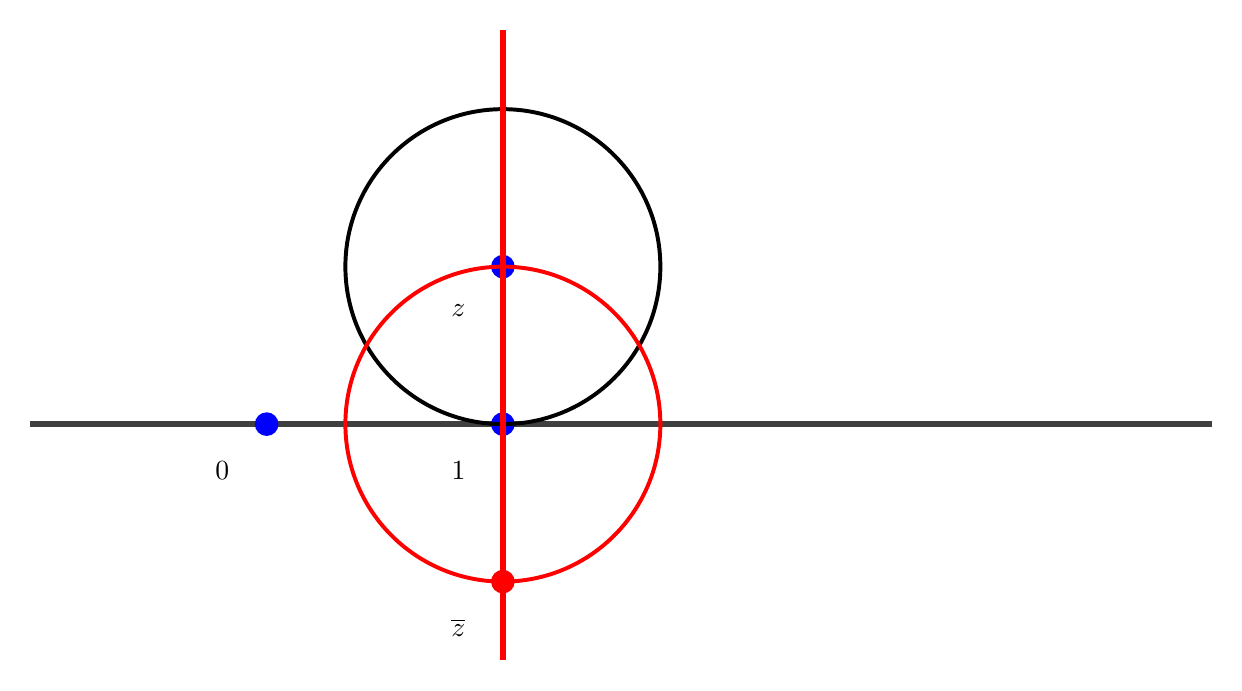
\begin{tikzpicture}
\draw[line width = 0.7mm, darkgray] (0,0) -- (15,0);
\fill[blue] (3,0) circle (0.15cm);
\fill[blue] (6,0) circle (0.15cm);
\fill[blue] (6,2) circle (0.15cm);
\node[below left=10pt] at (3,0) {$0$};
\node[below left=10pt] at (6,0) {$1$};
\node[below left=10pt] at (6,2) {$z$};
\draw[color=black, line width = 0.5mm] (6,2) circle [radius=2];
\draw[line width = 0.7mm, red] (6,-3) -- (6,5);
\draw[color=red, line width = 0.5mm] (6,0) circle [radius=2];
\fill[red] (6,-2) circle (0.15cm);
\node[below left=10pt] at (6,-2) {$\overline{z}$};
\end{tikzpicture}
\caption{- Example of case one of the proof of Lemma \ref{lemma:conjugate-in-Pn}}
\label{fig:case-1-conjugate}
\end{figure}
\FloatBarrier



\FloatBarrier
\begin{figure}[!hbt]
\centering
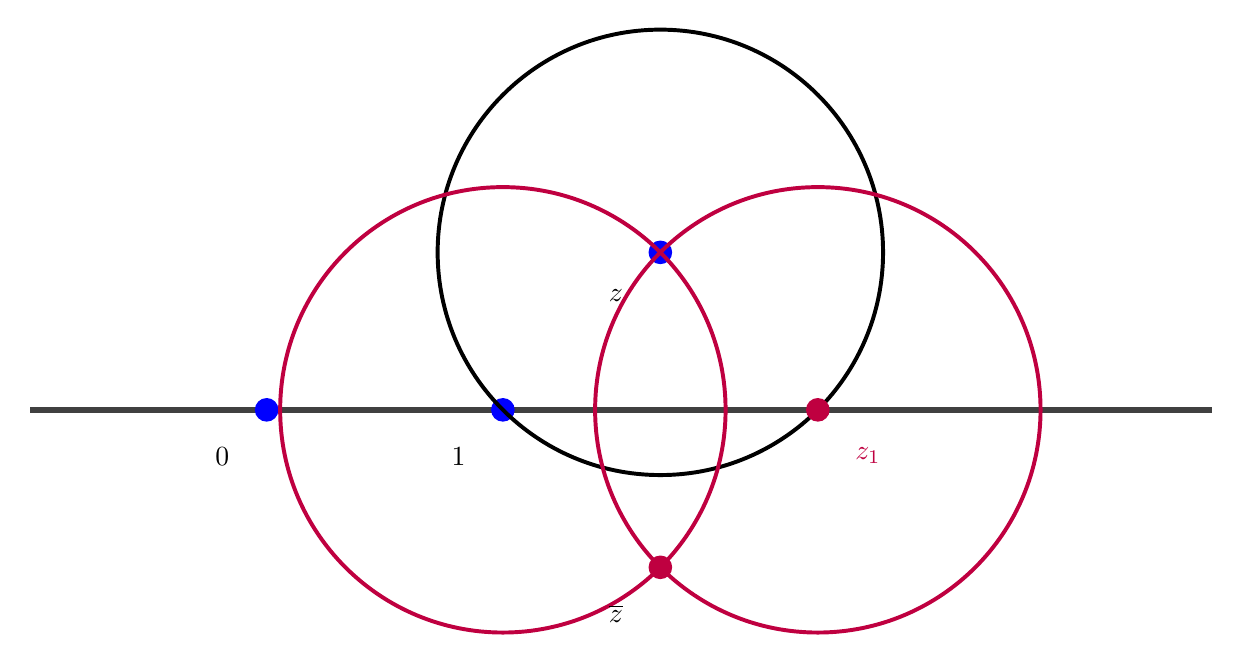
\begin{tikzpicture}
\draw[line width = 0.7mm, darkgray] (0,0) -- (15,0);
\fill[blue] (3,0) circle (0.15cm);
\fill[blue] (6,0) circle (0.15cm);
\node[below left=10pt] at (3,0) {$0$};
\node[below left=10pt] at (6,0) {$1$};
\fill[blue] (8,2) circle (0.15cm);
\node[below left=10pt] at (8,2) {$z$};
\draw[color=black, line width = 0.5mm] (8,2) circle [radius=2.828427];
\fill[purple] (10,0) circle (0.15cm);
\node[below right=10pt, color = purple] at (10,0) {$z_1$};
\draw[color=purple, line width = 0.5mm] (10,0) circle [radius=2.828427];
\draw[color=purple, line width = 0.5mm] (6,0) circle [radius=2.828427];
\fill[purple] (8,-2) circle (0.15cm);
\node[below left=10pt] at (8,-2) {$\overline{z}$};
\end{tikzpicture}
\caption{- Example of case two of the proof of Lemma \ref{lemma:conjugate-in-Pn}}
\label{fig:case-2-conjugate}
\end{figure}
\FloatBarrier

\begin{theorem}
    $\pi$ is not rational.
\end{theorem}

\begin{proof}

    \textcolor{red}{To Do:} Finish Proof
    Consider the following integral:

    $I_n = \int_{-1}^{1} (1-x^2)^ncos(\alpha x)dx$

    By integration by parts one time, we obtain that:

    $I_n = \frac{2n}{\alpha}\int_{-1}^{1}x\sin(\alpha x)(1-x^2)^{n-1}$
\end{proof}


\section{Diagrams}


\begin{figure}
	\centering
	\begin{tikzpicture}
		\draw[->, densely dotted] (-2.5,0) -- (2.5,0) node[below] {$\Re z$};
		\draw[->, densely dotted] (0,-2.5) -- (0,2.5) node[right] {$\Im z$};
		%		\draw[densely dotted] (0, 0) circle (1); 
		%		\draw[densely dotted] (0, 0) circle (1.26); 
		
		\fill (1.26, 0) circle (2pt) node[right] {$\sqrt[3]{2}$};
		\fill (-0.63, 1.09) circle (2pt) node[above] {$\zeta \sqrt[3]{2}$};
		\fill (-0.63, -1.09) circle (2pt) node[below] {$\zeta^2 \sqrt[3]{2}$};
		%		\fill (1, 0) circle (1pt) node[left] {$1$};
		%		\fill (-0.5, -0.866) circle (2pt) node[above] {$\zeta^ 2$};
		%		\fill (-0.5, 0.866) circle (2pt) node[below] {$\zeta$};
		\draw[->-=0.4, red] (1.26, 0) arc   (0:120:1.26)  node[midway] {$\tau$};
		\draw[->-=0.4, red] (-0.63, 1.09) arc (120:240:1.26)  node[midway] {$\tau$};
		\draw[->-=0.4, red] (-0.63, -1.09) arc (240:360:1.26) node[midway] {$\tau$};
		\draw[->-=0.5, blue] (-0.63, -1.09) to [out=120,in=240] node[right] {$\rho$} (-0.63, 1.09); 
		\draw[->-=0.5, blue] (-0.63, 1.09) to [out=300,in=60] node[right] {$\rho$} (-0.63, -1.09); 
		
		
		
		%		\draw[very thin,color=gray] (-3,-3) grid (3,3);
	\end{tikzpicture}
	\caption{Actions of $\tau$ and $\rho$ on the roots of $f(t) = t^3 - 2$.}
	\label{fig:example-action}
\end{figure}

\begin{figure}
	\centering
	\begin{tikzpicture}
		
		\node(A1) 										{\textcolor{blue}{$\Q(\zeta, \sqrt[3]{2})$}};
		\node(B1) [below left=2cm and 2cm of A1]      	{\textcolor{red}{$\Q(\zeta)$}}; 
		\node(B2) [below left=1cm and -0.7cm of A1]     {\textcolor{brown}{$\Q(\sqrt[3]{2})$}}; 
		\node(B3) [right=0.7cm of B2]					{\textcolor{orange}{$\Q(\zeta \sqrt[3]{2} )$}}; 
		\node(B4) [right=0.7cm of B3]					{\textcolor{purple}{$\Q(\zeta^2 \sqrt[3]{2} )$}}; 
		\node(C1) [below=3cm of A1]						{$\Q$}; 
		
		\draw[thick](A1) -- node[left]{3} (B1); 
		\draw[thick](A1) -- node[right]{2} (B2); 
		\draw[thick](A1) -- node[right]{2} (B3); 
		\draw[thick](A1) -- node[right]{2} (B4); 
		
		\draw[thick](C1) -- node[left]{2} (B1); 
		\draw(C1) -- node[left]{3} (B2); 
		\draw(C1) -- node[left]{3} (B3); 
		\draw(C1) -- node[left]{3} (B4); 
		
	\end{tikzpicture}
	\caption{Lattice diagram for intermediate fields of $\Q(\zeta, \sqrt[3]{2})$, where $\zeta = e^{2\pi i / 3}$. Each line from a lower field $K$ to an upper field $L$ indicates a field extension $L/K$. The number on each line indicates the degree of $L/K$, i.e. $[L:K]$. A thick line indicates that $L/K$ is a normal (and Galois) extension. }
	\label{fig:example-intermidate-fields}
\end{figure}

\begin{figure} 
	\centering
	\begin{tikzpicture}
		\node(A1) 										{\textcolor{blue}{$\langle e \rangle$}};
		\node(B1) [above left=2cm and 2cm of A1]      	{\textcolor{red}{$\langle \tau \rangle$}}; 
		\node(B2) [above left=1cm and -0.7cm of A1]     {\textcolor{brown}{$\langle \rho \rangle$}}; 
		\node(B3) [right=0.7cm of B2]					{\textcolor{orange}{$\langle \tau \rho  \rangle$}}; 
		\node(B4) [right=0.7cm of B3]					{\textcolor{purple}{$\langle \tau ^ 2 \rho  \rangle$}}; 
		\node(C1) [above=3cm of A1]						{$D_3$}; 
		
		\draw[thick](A1) -- node[left]{3} (B1); 
		\draw[thick](A1) -- node[right]{2} (B2); 
		\draw[thick](A1) -- node[right]{2} (B3); 
		\draw[thick](A1) -- node[right]{2} (B4); 
		
		\draw[thick](C1) -- node[left]{2} (B1); 
		\draw(C1) -- node[left]{3} (B2); 
		\draw(C1) -- node[left]{3} (B3); 
		\draw(C1) -- node[left]{3} (B4); 
	\end{tikzpicture}
	\caption{Lattice diagram for subgroups of $D_3$. Each line from a lower group $H$ to an upper group $G$ indicates that $H$ is a subgroup of $G$. The number on each line indicates the index of $H$ in $G$, i.e. $[G:H]$. A thick line indicates that $H$ is a normal subgroup of $G$. }
	 \label{fig:example-subgroups}
\end{figure}


		


